\documentclass[12pt]{article}

\usepackage{enumerate}
\usepackage{rotating}
\usepackage{multicol}
\usepackage{multirow}
\usepackage{graphicx}
\usepackage{fullpage}
\usepackage{subfigure}
\usepackage{setspace}
\usepackage{listings}
\usepackage{lastpage}
\usepackage{mathtools}
\graphicspath{{./images/}}

% for references
\usepackage[pagebackref=false,colorlinks,linkcolor=blue,citecolor=magenta]{hyperref}
\usepackage[nottoc]{tocbibind}
\usepackage{fancyhdr}
\setlength{\headsep}{25pt}

\pagestyle{fancy}
\fancyhf{}
\lhead{\lr{Digital Image Processing}}
\rhead{آزمون پایانترم}
\cfoot{صفحه \thepage\ از \pageref{LastPage}}
\lfoot{نیمسال مهر 00-99}
\rfoot{حمیدرضا ابوئی مهریزی}


% xepersian
\usepackage[extrafootnotefeatures]{xepersian}
\settextfont[Scale=1.2]{B Nazanin}
\setlatintextfont{Times New Roman}

\renewcommand{\labelitemi}{$\bullet$}

\begin{document}
	\doublespacing
	\begin{titlepage}
		\paragraph*{}
		\centering
			
			
			{\small به نام او}\\
			\vspace{1cm}
			\includegraphics[width=0.12\paperwidth]{aut.png}
			\hspace{2.5cm}
			%\includegraphics[width=0.15\paperwidth]{DIP}
			\hspace{2.5cm}
			\includegraphics[width=0.12\paperwidth]{bme}\\
			\vspace{2cm}
			{\Huge پردازش تصویر}\\
			\vspace{2cm}
			{\large استاد : دکتر حامد آذرنوش}\\
			\vspace{0.5cm}
			{\small  دانشجو :‌ حمیدرضا ابوئی}\\
			\vspace{0.5cm}
			{\small شماره دانشجویی : 9733002}\\
			\vspace{0.5cm}
			{\small آزمون پایانترم}\\
			\vfill
			{\tiny نیمسال مهر 00-99}
	\end{titlepage}
	\thispagestyle{plain}
	\tableofcontents
	\newpage
	%\onehalfspacing
	\doublespacing
	\section{سوال اول}
		\subsection{توضیحات تکمیلی روند کد}
			در قسمت آ برای یافتن هیستوگرام و اطلاعات مربوط به نویز تصویر روشی که استفاده شده است، جدا کردن قسمتی از تصویر که اطلاعات موبوط به نویز را در خود جای دهد. بدین منظور با توجه به تصویر داده شده، می‌توانیم اطراف تصویر که به نظر مشکی با نویز است انتخاب کنیم و اطلاعات مربوط به نویز را استخراج کنیم. نکته ای که وجود دارد آن است که هرچه تعداد داده های ما بیشتر باشد فراوانی دقیق تر و بهتر به دست می‌آید بنابراین در کد ، دو نوار سمت چپ و راست به قدری که وارد قسمت جمجمه نشود انتخاب شده و اطلاعات آن استخراج شد.
			
			از روی شکل نویز به دست آمده، به نظر می‌رسد که جنس تابع چگالی احتمال از جنس 
			\lr{Rayleigh}
			باشد.
			
			در قسمت و خواسته شده که بهبود برای کاهش نویز بررسی شود. همانطور که در تصویر خروجی و هیستوگرام آن مشخص است، میزان پراکندگی نویز در این حالت بسیار کمتر است. بنابراین می‌توان گفت که در نقاط غیر لبه ای، اثر نویز کاهش یافته است . البته در مکان هایی که ما تغییر داریم مانند لبه ها، چون حفظ اطلاعات برای ما ارزشمند است تغییراتی که اعمال میکنیم کمتر است و در آن نقاط نویز تصویر ما تغییر محسوسی نمی‌کند. اما لبه ها حفظ می‌شوند.
			
			روش میانه گیری با روش فیلتر تطبیقی یکسان عمل نمی‌کند زیرا روش میانه گیری کاری با محتوای درون کرنل ندارد و صرفا به این که داخل هر کرنل مقدار میانه چه عددی است کار دارد. اما در روش فیلتر تطبیقی ، محتوای داخل کرنل اهمیت می‌یابد. بدین صورت که میزان واریانس و میانگین نقاط داخل کرنل  روی میزان کاهش نویز تاثیر دارد. بنابراین زمانی که به خروجی نگاه میکنیم در نقاطی که ما اطلاعات مهم داریم ،در روش میانه گیری این اطلاعات از بین می‌روند ولی در روش فیلتر تطبیقی این اطلاعات مهم از بین نمی‌روند. اما صرفا از دید کاهش نویز ،فیلتر میانه بهتر عمل می‌کند اما هوشمندانه خیر.
			
			البته لازم به ذکر است که هنگام پیاده سازی فرمول این فیلتر که برابر است با 
$f(x,y) = g(x,y) - \frac{\sigma^2_\eta}{\sigma^2_L}[g(x,y) - m_l]$
و اگر همینجوری فقط واریانس پنجره ها را در فرمول بگذاریم، به مشکلاتی بر می‌خوریم. برای مثال مشاهده می‌کنیم که مقادیر منفی در نتیجه آمده است. با بررسی مجدد متوجه می‌شویم که باید این واریانس ها و واریانس کلی را به روشی مناسب تر به دست آوریم؛ بدین صورت که ابتدا واریانس هر پنجره را به دست می‌آوریم. سپس 
$\sigma^2_\eta$
برابر است با میانگین واریانس های پنجره ها. سپس برای منفی نشدن مقادیر، واریانس هایی که کمتر از واریانس $\eta$ است را برابر با واریانس $\eta$
می‌گذاریم و با این مقادیر فرمول بالا را پیاده سازی می‌کنیم

		\subsection{ورودی برنامه}
		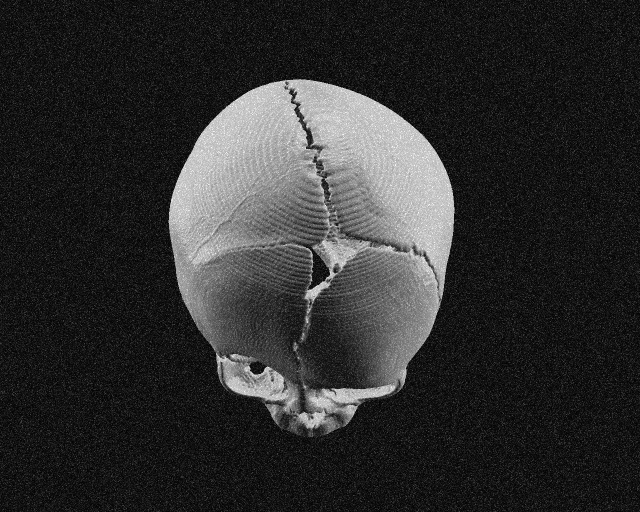
\includegraphics[width=10cm]{inputs/noisy_skull.png}
		\subsection{خروجی برنامه}
		\lr{Mean of noise is:      19.9309765625\\
			Variance of noise is:  129.10471493174234\\}
		
		\includegraphics[width=13cm]{1-0}\\
		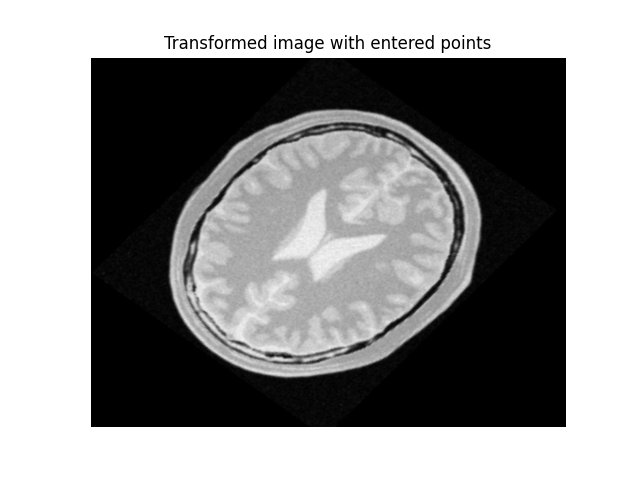
\includegraphics[width = 17 cm]{1-1}\\
	%	\includegraphics[width = 17 cm]{1-2}
		
		
		\newpage
		
		\section{سوال دوم }
		\subsection{توضیحات تکمیلی روند کد}
	با بررسی بیشتر تصویر مشاهده میکنیم که با این که تصویر نسبتا به صورت باینری است ، اما وجود برخی نویز های بسیار کوچک ممکن است کار ما را خراب کند بنابراین ابتدا با یک ترشهولد گیری آن را کاملا باینری می‌کنیم.
	
	برای گرفتن موقعیت کلیک کاربر از 
	\lr{plt.canvas.mpl\_connect}
	استفاده شده است. همچنین برای بررسی این که آیا دکمه ی اسکیپ زده شده یا خیر نیز می‌توان از این استفاده کرد که کد آن در تابع \lr{esc}
مشخص است.
هنگامی که تابع پر کردن حفره فراخوانی می‌شود و مختصات در ورودی داده می‌شود، به سراغ اعمال الگوریتم می‌رویم. در اینجا ما با دایلیت کردن با کرنل + ، همسایگی نقاط اولیه خود را می‌یابیم. سپس با بررسی این که آیا این نقاط داخل تصویر اصلی نیز سفید هستند یا خیر؛ متوجه می‌شویم که آیا این نقاط جدید را باید به ناحیه ی خود اضافه ‌کنیم یا خیر. سپس مجددا همین مسیر را پیش می‌رویم تا جایی که با دایلیت کردن و مقایسه ناحیه ی جدید، دیگر هیچ پیکسل جدیدی به ناحیه ی ما اضافه نشود. حال همان تصویر را که در این جا به صورت گلوبال مشاهده کردیم تغییر می‌یابد و پس از اتمام حلقه، نسخه ی جدید آن را مشاهده می‌کنیم.
	
		\subsection{ورودی برنامه}
		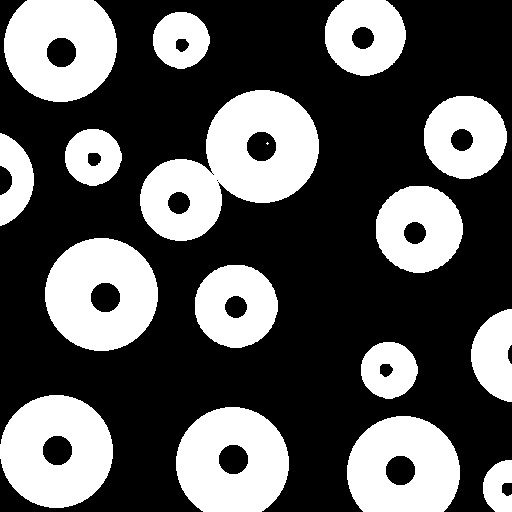
\includegraphics[width=5cm]{inputs/reflections.jpg}\\
	%	\includegraphics[width=5cm]{inputs/CT_2.png}
		\subsection{خروجی برنامه}
		
	 با کلیک روی مرکز های دایره ها به راحتی تصویر زیر به دست می‌آید\\
		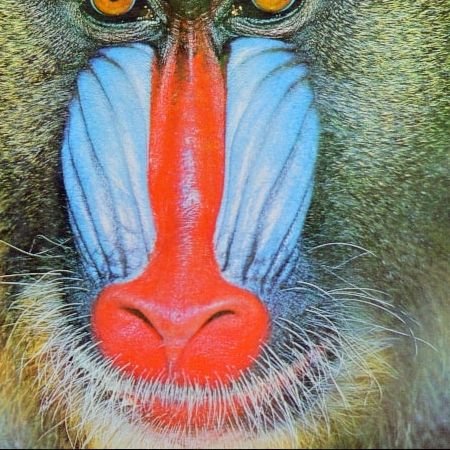
\includegraphics[width=15cm]{2.png}
	%	\includegraphics[width=8cm]{2-3.png}
		
		\newpage
		
		\section{سوال سوم }
		\subsection{توضیحات تکمیلی روند کد}
	برای یافتن تصویر پس زمینه می‌توان از راه های مختلف استفاده کرد. یکی از راه ها استفاده از میانگین تصاویر است. راه دیگری که می‌توان پس زمینه را به دست اورد و در کد موجود است استفاده از میانه است بدین صورت که تمام ویدیو را در یک لیست می‌گذاریم و سپس در محور زمان از آن با استفاده از تابع مدین بکگراند را استخراج می‌کنیم . این روش بهتر از روش قبل کار می‌کند و نتیجه ی بهتری دارد زیرا در حالت اول تمام تحرک ها در بکگراند ما تاثیر می‌گذاشتند. 

حال می‌توانیم مجددا فیلم را بازخوانی کنیم و در همین حین، بکگراند را از آن کم کنیم و جاهایی که تفاوت زیادی دارد. بدین معناست که یه شی در حال جابجایی است. حال برای این که اشیا در حال جابجایی را با رنگ قرمز مشخص کنیم ابتدا قسمت هایی که در حال تغییر است را صفر می‌کنیم و سپس درآن قسمت ها رنگ قرمز را اضافه می‌کنیم تا نتیجه نهایی به دست بیاید. 
		\subsection{ورودی برنامه}
		\includegraphics[width=12cm]{inputs/frame89.jpg}
		\subsection{خروجی برنامه}
		\includegraphics[width=12cm]{frame89.png}\\
		پس زمینه ی دیتکت شده به صورت زیر است :\\
		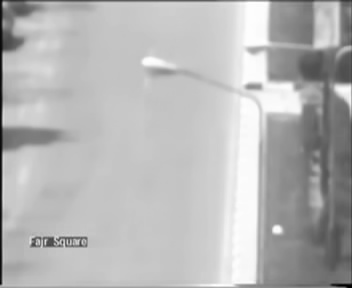
\includegraphics[width=12cm]{background.jpg}
		
		\newpage
		
		\section{سوال چهارم }
		\subsection{توضیحات تکمیلی روند کد}
	 در این سوال برای یافتن پاسخ نهایی ابتدا با استفاده از همان روش 
	 \lr{plt.canvas.mpl\_connect}
	 مختصات نقطه‌ی دانه را از کاربر می‌گیریم سپس وارد تابع می‌شویم. میخواهیم ناحیه ی یافته شده را در یک تصویر مشکی با ابعاد تصویر اصلی نشان دهیم. 
	 (\lr{black})
	
	 سپس در این سوال دایلیت میکنیم و هر سری بررسی میکنیم که آیا پیکسل های جدید که به دست آمده اند، داخل سگمنت قرار می‌گیرند یا خیر. این مقایسه می‌تواند به شکل‌های متفاوتی صورت گیرد. اگر ما هر سری که دایلیت میکنیم و همسایگی های ۴ یا ۸ تایی (برای مشخص کردن این که در حال استفاده از کدام هستیم کرنلمان را با توجه به متغیر
	 \lr{neighberhood\_4}
	به دست می آوریم ) 
	را با پیکسل کناری که دایلیت شده است مقایسه کنیم، اتفاقی که رخ می‌دهد نشت کردن است. یعنی به مرور ممکن است سطح چیزی که مقایسه میکنیم تغییر محسوسی کند. بدین منظور می‌توانیم از راه های دیگری برای جلوگیری از این اتفاق استفاده کنیم. برای مثال کلا شدت پیکسل انتخاب شده توسط کاربر را ملاک در نظر بگیریم و یا این که میانگین شدت های پیکسل‌های داخل محدوده را به عنوان ملاک شباهت یابی در نظر بگیریم که خوبی این روش این است که محدوده ی انتخاب شده بسیار خوب و دقیق تر از حالت قبل انتخاب می‌شود. حال باید در پیکسل های جدید بگردیم و این 
	\lr{thresholding}
	را در مقایسه با ملاکی که بالاتر توضیح داده شد بگیریم و اگر قدر مطلق تفاوت ها کمتر از سطح داده شده(11) باشد، پیکسل داخل محدوده است و جزو پیکسل های سگمنت شده محسوب می‌شود. این کار را می‌توان به این صورت انجام داد که در هر ایتریشن، یک بار کل پیکسل های تصویر را بخوانیم و اگر جزو پیکسل های جدید بود، شرط بودن در سگمنت را بررسی کنیم. اما این روش بهینه نیست و زمان زیادی طول می‌کشد مخصوصا اگر سگمنتی که قرار است انتخاب شود، بزرگ باشد و نیاز به ایتریشن زیادی داشته باشد (همانطور که در سوال ۲ نیز مطرح شد، هنگامی که تعداد پیکسل های سگمنت در یک ایتریشن تغییر نکند متوجه می‌شویم که کار سگمنتیشن به پایان رسیده است) 
	
	حال الگوریتمی که می‌توان استفاده کرد برای این که سرعت را بهبود دهیم این است که از برخی روش ها و توابع پایه و معمولی نامپای که در تمام کد ها استفاده می‌کردیم ، استفاده کنیم و تغییر خیلی کوچکی در بررسی شرط بودن در سگمنت انجام دهیم که در ادامه به توضیح آن می‌پردازیم.
	
	همانطور که در بالا گفتیم ابتدا شاخص که همان میانگین پیکسل های داخل سگمنت هست را در نظر میگیریم. سپس پیکسل هایی که قرار است چک شوند (دایلیت شده ی سگمنت منهای خود سگمنت برای به دست آوردن پیکسل های جدید) را ابتدا در تصویر می‌یابم و آن را از شاخص کم میکنیم . بدین ترتیب برای مثال اگر شاخص ما ۶۰ باشد، تصویر ما از ۰ تا ۲۵۵ به -۶۰ تا ۱۹۵ تغییر می‌یابد. حال از این تصویر قدر مطلق میگیریم. بدین ترتیب تصویر ما به ۰ تا ۱۹۵ تبدیل می‌شود که مقادیر منفی مثبت شده اند. حال ترشهولدینگ را با قطع از سطح ترشهولد داده شده (11) انجام می‌دهیم. حال این ترشهولد شده را ابتدا معکوس می‌کنیم بدین صورت که مقادیر ۰ تا سطح ترشهولد(۱۱) ماکزیمم و مقادیر بیشتر، صفر شوند. حال این ترشهولد گرفته شده را با نقاط جدید 
	\lr{and}
	می‌کنیم و نقاطی که به دست می‌آید، پیکسل های جدید صدق شده در شرط است و حال این نقاط را به نقاط سگمنت شده اضافه می‌کنیم. همانطور که مشاهده می‌شود در این روش ما تک تک نقاط تصویر را یک به یک بررسی نکردیم بلکه برای تصویرمان یک الگوریتم یافتیم که سرعت را چندین برابر زیاد می‌کند. 
	همچنین در کد یک پرچم تعریف شده است که عملیات فقط بار اول که تصویر داریم اجرا شود و اگر دفعات بعد کلیک کردیم اتفاقی نیافتد

		\subsection{ورودی برنامه}
		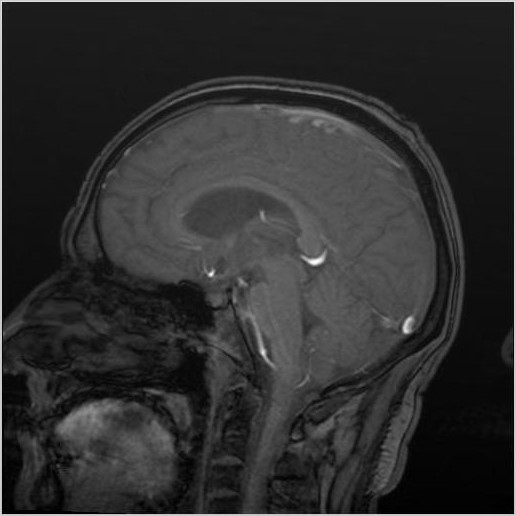
\includegraphics[width=10cm]{inputs/fMRI.jpg}		
		\subsection{خروجی برنامه}
		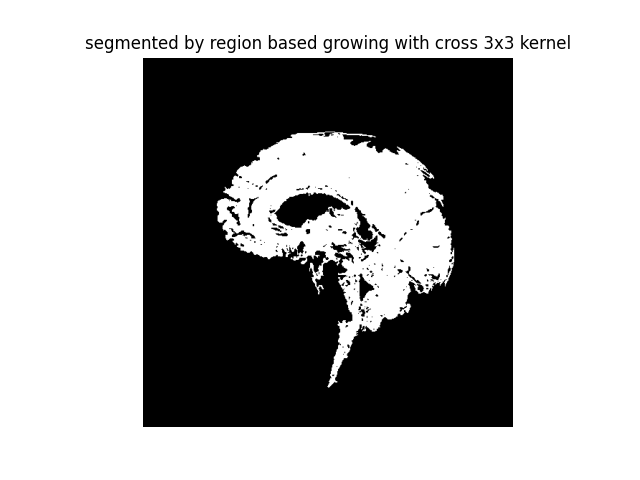
\includegraphics[width=15cm]{out4.png}\\
		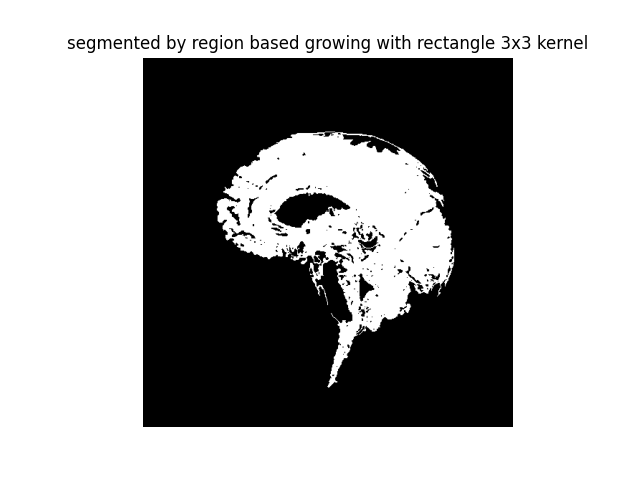
\includegraphics[width=15cm]{out8.png}


\end{document}
